\documentclass[crop,tikz]{standalone}
\usetikzlibrary{%
    arrows,
    arrows.meta,
    backgrounds,
    calc,
    decorations.pathreplacing,
    fit,
    matrix,
    positioning,
    scopes,
    shadows
}
\usepackage[linguistics]{forest}
\usepackage[charter]{mathdesign}
\tikzset{headarrow/.style = {-{Latex[length=.5em]}}}
\newcommand{\setof}[1]{\ensuremath{\left \{ #1 \right \}}}

\begin{document}
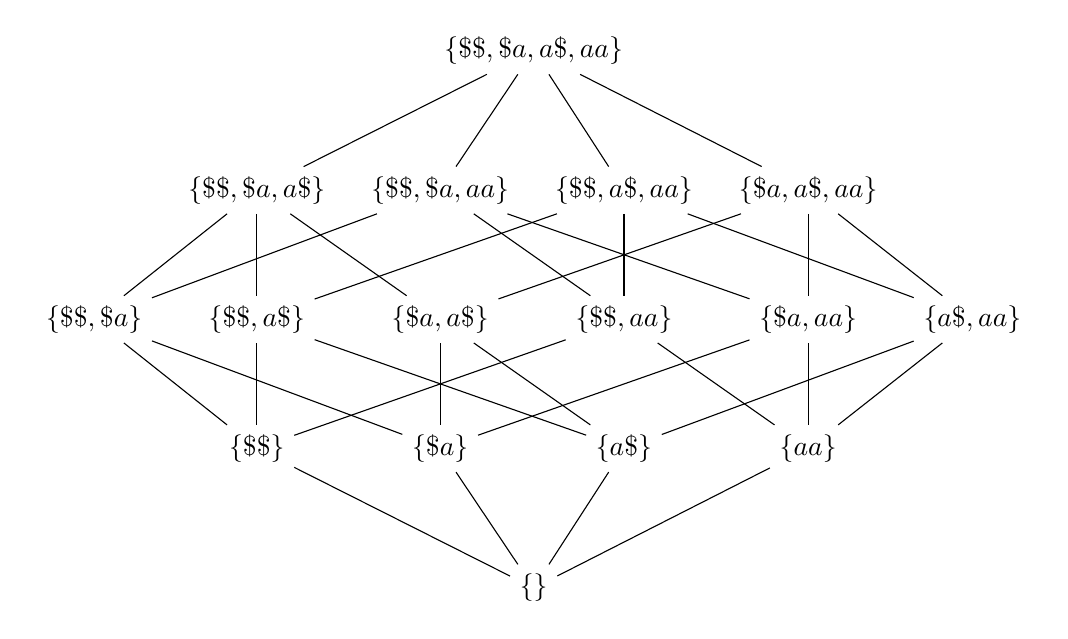
\begin{tikzpicture}
    \matrix (m) at (0,0) [matrix of math nodes,
                      row sep=3em, column sep=1em] {
                      & \setof{\$\$, \$a, a\$} & \setof{\$\$, \$a, aa} & \setof{\$\$, a\$, aa} & \setof{\$a, a\$, aa} & \\
    \setof{\$\$, \$a} & \setof{\$\$, a\$}      & \setof{\$a, a\$}      & \setof{\$\$, aa}      & \setof{\$a, aa}      & \setof{a\$, aa}\\
                      & \setof{\$\$}           & \setof{\$a}           & \setof{a\$}           & \setof{aa}           & \\
    };
    \node (top) [above=3em of m.north] {$\setof{\$\$, \$a, a\$, aa}$};
    \node (bot) [below=3em of m.south] {$\setof{}$};

    \foreach \Source/\Target in {%
        3-2/2-1,
        3-2/2-2,
        3-2/2-4,
        3-3/2-1,
        3-3/2-3,
        3-3/2-5,
        3-4/2-2,
        3-4/2-3,
        3-4/2-6,
        3-5/2-4,
        3-5/2-5,
        3-5/2-6,
        1-2/2-1,
        1-2/2-2,
        1-2/2-3,
        1-3/2-1,
        1-3/2-4,
        1-3/2-5,
        1-4/2-2,
        1-4/2-4,
        1-4/2-6,
        1-5/2-3,
        1-5/2-5,
        1-5/2-6%
    }
    \draw (m-\Source) to (m-\Target);
    \foreach \Column in {2,3,4,5}
        {
            \draw (m-1-\Column) to (top);
            \draw (m-3-\Column) to (bot);
        }
\end{tikzpicture}
\end{document}
